\documentclass{amsart}
\usepackage{hyperref}
\usepackage{graphicx}

\DeclareMathOperator{\Galways}{\mathbf{G}}
\DeclareMathOperator{\Feventually}{\mathbf{F}}
\DeclareMathOperator{\Xnext}{\mathbf{X}}
\DeclareMathOperator{\Uuntil}{\mathbf{U}}

\theoremstyle{definition}
\newtheorem{example}{Example}[section]


\begin{document}
\title{A competition on formal methods for robotics}
\author{Scott C. Livingston}
\author{Vasumathi Raman}
\date{24 Sep 2014}
\begin{abstract}
This is the normative reference for the first challenge on formal methods for
robotics.  Formal methods refers broadly to techniques for the verification and
automatic synthesis of transition systems that satisfy desirable properties
exactly or within some statistical tolerance.  Though historically developed for
concurrent software, recent work has brought these methods to bear on motion
planning in robotics.  Challenges specific to robotics, such as uncertainty and
real-time constraints, have motivated extensions to existing methods and
entirely novel treatments.  However, compared to other areas within robotics
research, demonstrations of formal methods have been surprisingly small-scale.
The proposed robotics challenge seeks to motivate advancement of the state of
the art toward practical realization.  The challenge is organized into three
problem domains: arbitrary dimensional double integrators, roads with Dubins
cars, and manipulation tasks on the assembly line.
\end{abstract}
\maketitle


\section{Introduction}

We present the first challenge on formal methods for robotics, which will
henceforth be referred to simply as ``the Challenge.''  It is to be hosted at
the International Conference on Robotics and Automation ({ICRA}) in May 2015.
The purpose of this document is to describe in detail the Challenge, including
the problem domains, rules, and scoring procedures.  Unless explicitly stated
otherwise, the description herein is normative.

\section{Summary}

The challenge will consist of three problem domains that touch on a diversity of
difficulties one would need to address in a practical deployment.  These problem
domains together involve many fronts of current work in formal methods for
robotics.  To avoid requiring too general of a solution---and in particular, to
improve accessibility for a broad group of potential competitors---entries to
the challenge are permitted to select a subset of these domains.  More
precisely, each team may enter any number of control programs, each of which may
be used on any subset of the problem domains.  Results of the challange will be
organized by problem domains.  Control programs that are used in multiple
domains will receive total scores as the sum of scores from each attempted
domain.  The intent in the scoring structure will be to have excellent
performance in a single problem domain regarded as being comparable to good
performance in all domains.  Teams will be able to trade-off generality with
problem-specific tuning.

In the preparation materials to be made available for potential competitors, we
will release elementary solutions to complete each domain.  These will establish
feasibility of the problems, provide reference implementations for the challenge
execution framework, and give teams something on which to build, should they
choose to do so.


\section{Preliminaries}

We briefly present basic concepts and notation that may not be widely known by
potential participants at ICRA.  Linear temporal logic (LTL) is an extension of
boolean (or propositional) logic that describes properties for countably
infinite sequences of events.  Within this proposal, the most relevant is $\psi
\Uuntil \varphi$, which informally requires that the formula $\psi$ holds until
a state satisfying $\varphi$ is reached.  The operator $\Galways$ is also used;
informally, $\Galways \psi$ requires $\psi$ is satisfied by all states reached
during an execution.  Intuitively the operator $\Feventually$ is dual to
$\Galways$; informally, $\Feventually \psi$ requires that a state satisfying
$\psi$ occurs in finite time.

A convex polytope is a bounded region defined by the intersection of finitely
many halfspaces, each of which is defined by a linear inequality.  There are
many useful computations known for polytopes, many of which are fast, e.g.,
intersection. \cite{Fukuda2004}

The discrete notions of temporal logic are related to the real-valued spaces of
continuous dynamical systems as follows.  Suppose a state space contains
finitely many polytopes, and each polytope is regarded as labeled.  A trajectory
through this space is labeled with the sequence of polytopes with which it
intersects.


\section{Problem domain: Scaling double-integrators}\label{sec:scalingdoubleinteg}

The first problem domain is the simplest in terms of dynamics and
specifications, yet unlike the other domains, the system to be controlled can be
scaled easily to arbitrarily many dimensions.  While this problem is abstract in
the sense that it is not modeling a specific physical system, it is
well-motivated because the double-integrator is just the basic force equation
($F=ma$) of Newtonian mechanics, up to a scaling factor.  In other words, this
problem domain concerns acceleration of a point-mass in high-dimensional spaces
so as to visit goal regions and avoid obstacles.  The precise description is
given below.

\subsection{Dynamics and constraints}

Let $n$ be a positive integer.
\begin{equation}\label{eq:doubleinteg}
\ddot{q} = u ,
\end{equation}
where $q(t)\in \mathbb{R}^{n}$ and $\dot{q}(t)$ are called the \textit{position}
and \textit{velocity}, respectively, at time~$t$.  The input is bounded as
$\lVert u(t) \rVert_1 \leq u_{\mathrm{max}}$.  To introduce process and sensor
noise, consider the 2-dimensional system
\begin{align}
\dot{x} &= \left(
\begin{array}{cc}
0 & 1 \\
0 & 0
\end{array}
\right) x + \left(
\begin{array}{c}
0 \\
1
\end{array}
\right) u + \xi \label{eq:dintegdyn}\\
y &= \left(
\begin{array}{cc}
1 & 0
\end{array}
\right) x + \eta \label{eq:dintegobs},
\end{align}
where $\xi$ and $\eta$ are either bounded disturbances (nondeterministic) or
stochastic processes.  Equivalence with \eqref{eq:doubleinteg} in the case of
$n=1$ and $\xi=\eta=0$ is apparent using $x_1 = q$ and $x_2 = \dot{q}$.  For $n
> 1$, the matrices in \eqref{eq:dintegdyn} and \eqref{eq:dintegobs} can be
repeated in block diagonal form to yield a new linear time-invariant system of
dimension $2n$ and which is again equivalent to \eqref{eq:doubleinteg}.

For this aspect of the ``scaling double-integrators'' problem domain, we are
able to vary the number of position dimensions $n$, the maximum 1-norm of the
control input $u_{\mathrm{max}}$, and the process and sensor noise $\xi$ and
$\eta$.

\subsection{Specifications}

Task specifications will require visitation of regions while avoiding obstacles.
Compared with the specifications for the other problem domains presented in
Sections~\ref{sec:trafficdubins} and \ref{sec:dexterousmanip}, these can be
regarded as a slight extension beyond classical motion planning.  There are two
forms of specifications:
\begin{equation}\label{eq:dinteg-surveillance}
q(0) = \mathrm{init} \wedge \Galways \left( q(t) \notin \mathrm{Obs} \right) \wedge \bigwedge_{i} \Galways \Feventually \mathrm{goal}_i
\end{equation}
and
\begin{equation}\label{eq:dinteg-timedreach}
q(0) = \mathrm{init} \wedge \Galways \left( q(t) \notin \mathrm{Obs} \right) \wedge \bigwedge_{i} \left( \mathrm{counter}_i \leq T_{i} \right) \Uuntil \mathrm{goal}_i ,
\end{equation}
where $\mathrm{Obs} \subset \mathbb{R}^n$ is the obstacle set, which is
represented by a finite union of polytopes.  For each $i$, $\mathrm{counter}_i$
is a discrete clock that enforces the real-time deadline $T_i$ of reaching
region $\mathrm{goal}_i$.  Goal region $\mathrm{goal}_i$ is defined by a convex
polytope.  The initial position is a single point, $\mathrm{init}\in
\mathbb{R}^n$.  As part of the specification form \eqref{eq:dinteg-timedreach},
a time of initialization and rate of progression of the discrete counters is
specified.  These are significant because they determine in what order and how
quickly the goal regions must be reached.

\subsection{Implementation plan for the challenge}

This problem domain will be evaluated entirely within a numerical simulation.
As such, competitors will submit controllers for this part of the challenge
before the conference, and results will be obtained during live runs at ICRA.
After completion of each run in real-time, using software released as part of
the problem domain source code, animations will be generated to depict results.
The main evaluation metric for this domain will be scalability of solutions to
high dimensions and large problem sizes. As such, we are currently investigating
feasibility of running the trials for this domain on common compute hardware,
such as through Amazon Web Services (\url{http://aws.amazon.com/}).


\section{Problem domain: Traffic network of Dubins cars}\label{sec:trafficdubins}

This domain involves navigation in a small network of two-lane roads with
vehicles that follow unicycle-like dynamics. Unlike the ``scaling
double-integrators'' problem (cf.\ Section~\ref{sec:scalingdoubleinteg}), now
there is an adversary that selects the motion of other cars.  The adversary is
subject to assumptions such as obeying traffic rules and not parking unfairly at
locations that must be eventually reached by the controller.

\subsection{Dynamics and constraints}
All cars including the controlled robot are assumed to have the same rigid body
shape and to have the same dynamics. Let $\mathcal I$ be the index set for the
cars in the network, with $r$ denoting the index of the controlled robot; all
cars indexed with $i \in {\mathcal I}\backslash\{r\}$ are regarded as a part of
the (adversarial) environment.

The pose of each car $i \in {\mathcal I}$ is specified by $(x_i,y_i,\theta_i)$,
where $(x_i,y_i)\in \mathbb{R}^2$ is referred to as \textit{position}, and
$\theta_i \in S^1$ is referred to as \textit{orientation}.  The car's body is a
rectangle or a circle, and the position is defined to be at the mean point
(center of mass) of the body.  Let $w$ be the width of the car -- this is
identical for each $i \in {\mathcal I}$.

The trajectories of car $i$ are solutions of
\begin{align}
\dot{x_i} &= u_i \cos \theta_i \\
\dot{y_i} &= u_i \sin \theta_i \\
\dot{\theta_i} &= \omega_i
\end{align}
where the control inputs are constrained as $u_i(t)\in \{0,u_{\mathrm{max}}\}$ and
$\omega_i(t) \leq \omega_{\mathrm{max}}$.


The workspace is a randomly generated road network constructed as follows.
Create a planar graph $G = (V,E)$ in which each vertex $v$ has degree $d_v \le 4$
(i.e., at most 4 neighbors).  Embed this graph in the plane, and expand the
edges to have width $4w$ (recall $w$ is the common vehicle width).

For this aspect of the ``traffic network of Dubins cars'' problem domain, we are
able to vary the bounds $u_{\mathrm{max}}$ and $\omega_{\mathrm{max}}$ on the
permissible control inputs, the size ($|V|$) and topology ($|E|$) of the road
network, and the number of other cars, i.e. $|\mathcal I|$.


\subsection{Specifications}

Because there is now an environment that may behave adversarially, task
specifications will be of the form $\varphi_{\mathrm{env}} \Rightarrow
\varphi_{\mathrm{sys}}$, where $\varphi_{\mathrm{env}}$ is known as the
``assumption'' and $\varphi_{\mathrm{sys}}$ as the ``guarantee.''  The desired
behaviors to be realized by the robot are provided through
$\varphi_{\mathrm{sys}}$ and include
\begin{enumerate}
\item obstacle avoidance while repeatedly visiting regions of interest, as in
  \eqref{eq:dinteg-surveillance};

\item reaching certain points within a time limit, e.g., as a model of deadlines
  for refueling, as in \eqref{eq:dinteg-timedreach};

\item remaining in the right-lane except when it is blocked;

\item stopping at intersections, which are treated as all-ways stops, and then
  proceeding based on order of arrival.
\end{enumerate}
The other cars will be assumed to follow the same road rules as listed above.
However, exceptions (violations) may occur, and thus additional fairness
assumptions will be provided, e.g.,
\begin{equation}\label{eq:freegoals}
\bigwedge_i \Galways \Feventually \tt{free}(\mathrm{goal}_i)
\end{equation}
which provides that other cars will always eventually vacate the $i$-th goal
region.

\begin{figure}[h!]\label{fig:network}
  \centering
        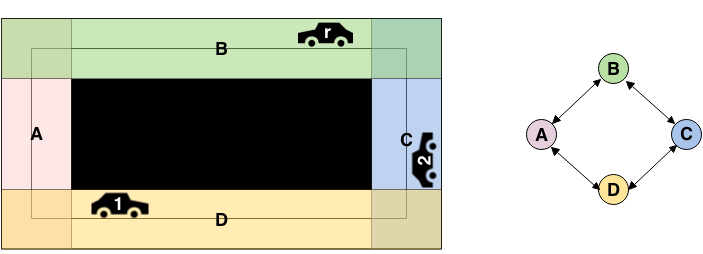
\includegraphics[width=1.0\textwidth]{images/network}
  \caption{An example road network and the graph from which it was generated. There are three cars, one of which is the robot (labeled with $r$)}.
\end{figure}

\begin{example}
Consider the network depicted in Fig. \ref{fig:network}. There are three cars,
one of which is the robot to be controlled. The road network graph is depicted,
and shows the bidirectional connectivity between the four road segments $A$,
$B$, $C$ and $D$. Note that each road has two lanes. At the intersection of each
pair of roads, there is an overlap region.
\end{example}

TODO: what does the LTL specification look like for this problem?

\subsection{Implementation plan for the challenge}

We are currently exploring feasibility of simulation using CloudSim
(\url{http://cloudsim.io}), which was developed for running Gazebo-based
simulations (\url{http://gazebosim.org}) as part of the ``virtual'' component of
the current DARPA challenge (\url{http://www.theroboticschallenge.org}).

Besides simulation, we plan to construct a reduced size form of this challenge
domain for running on-site at ICRA.  Both the robot to be controlled and the
adversarial vehicles will be based on Kobuki mobile bases
(\url{http://yujinrobot.com/eng/?portfolio=kobuki}).  Because all
problem-relevant motion will occur within a fixed plane, high-speed overhead
pose tracking is possible using a single camera mounted on the ceiling.  We hope
to install such a system on-site at ICRA to provide ground truth positions for
scoring purposes, even if the data is not available to competitors during the
challenge.

\section{Problem domain: Dexterous manipulation on the assembly line}\label{sec:dexterousmanip}

This problem domain concerns pick and place tasks, expressed using LTL
contracts, as described below. The key challenges explored in this problem
domain will include uncertainty in the shape and dynamics of the end-effector,
as well as objects that are being grasped, and collision-avoidance with moving
obstacles that come into the workspace, including humans.

For the tasks in this problem domain, the robot workspace is a three-dimensional
Euclidean space. We will consider two dynamic settings: one in which the working
surface is moving, and one in which it is not.  The former is motivated by
conveyor belts, and tasks that may be expected in an assembly line. The focus is
on moving objects around or performing end-effector specific behaviors, but will
not involve difficult grasping problems, like deformable surfaces.

For each end-effector, we will provide a description of its shape and how to use
it, i.e.  how it should be positioned relative to the items of interest so that
an abstract ``execute-end-effector'' action can be taken. For example, in order
for a paint spraying device to be used, it should have a certain proximity to
the object-to-be-sprayed, and a minimum distance from objects that should be
left unpainted. These requirements would be expressed using LTL. Besides shape,
the dynamics of the arm (without any end-effector) would be affected by the
end-effector -- these modified dynamics would also be provided.

Finally, these tasks will be reactive, in that they will involve an adversary
that can interfere with the workspace. Assumptions on this adversary and how it
can affect the workspace will also be provided.

\subsection{Implementation plan for the challenge}

We are exploring several simulation environments for this domain, including the following.
\begin{itemize}
\item Gazebo (\url{http://gazebosim.org/})
\item OpenGRASP (\url{http://opengrasp.sourceforge.net/})
\item Peter Corke's Robotics Toolbox
(\url{http://petercorke.com/Robotics_Toolbox.html})
\item Klamp't (\url{http://www.iu.edu/~motion/klampt/})
\end{itemize}

We are also still exploring the possibility of a physical testbed on-site at ICRA.


\bibliographystyle{abbrv}
\bibliography{fmrchallenge.bib}

\end{document}
